\documentclass[10pt,journal,compsoc]{IEEEtran}
\def\code#1{\texttt{#1}}

\ifCLASSINFOpdf
  \usepackage{graphicx}
  \graphicspath{{Figures/}{Other_Folder/}}
  \DeclareGraphicsExtensions{.pdf,.jpeg,.png}
\else
\fi
\ifCLASSOPTIONcompsoc
 \usepackage[caption=false,font=footnotesize,labelfont=sf,textfont=sf]{subfig}
\else
 \usepackage[caption=false,font=footnotesize]{subfig}
\fi
\usepackage{url}
\usepackage{hyperref}
\usepackage{listings}
\usepackage{color}
\usepackage{caption}
\usepackage{biblatex}
\addbibresource{bibliography.bib} 
\definecolor{dkgreen}{rgb}{0,0.6,0}
\definecolor{gray}{rgb}{0.5,0.5,0.5}
\definecolor{blue}{rgb}{0.0,0.0,1.0}
\lstset{frame=tb,
  language=C,
  aboveskip=3mm,
  belowskip=3mm,
  showstringspaces=false,
  columns=flexible,
  basicstyle={\small\ttfamily},
  numbers=none,
  keywordstyle=\color{blue},
  commentstyle=\color{dkgreen},
  stringstyle=\color{gray},
  breaklines=true,
  breakatwhitespace=true,
  tabsize=4,
  numbers=left,
  stepnumber=1,    
  firstnumber=1,
  numberfirstline=true,
  xleftmargin=5.0ex,
}
\newcommand{\comment}[1]{}

\hyphenation{}

\begin{document}

\title{Performance Impact of \textit{CUDA} on Image Manipulation Algorithms}

\author{Luis Silva - 54449,
        Lourenço Soares - 54530%
}

\markboth{December~2021}{}

% make the title area
\maketitle

\IEEEraisesectionheading{\section{Introduction}\label{sec:introduction}}

\IEEEPARstart{T}{his} report intends on investigating the impact of optimizations and implementations using CUDA on the processing time of image manipulation algorithms, which we will refer to as shaders (because that is, in essence, what the two algorithms are). This program in question implements two effects, the first being a blur operation (which requires reading neighboring "pixels") and the second being a color correction (desaturation) shader. \\

\noindent We attempted to iterate on our solutions, experimenting with different approaches to setting up tasks and memory for the GPU in order to minimize the time spent performing the effects, and compared the results (which were obtained both with basic CPU timers and with a heavier tool like nvprof) with previous solutions. 


\section{Approach and Results}

\noindent The programs used to benchmark different implementations, which are mentioned throughout this section, as well as the results obtained from them, can be downloaded from our public \textit{Git} repository\cite{projectrepo}. The times given in this section were obtained via our autotester program, which tested each version of our implementations 10 times with the \code{tram.ppm} image on the University's cluster.


\subsection{Original Code}

\noindent First and foremost, after reading the original source code that was provided to us by the professor, we saw some improvements that could be made to the program in order to substantially reduce the time spent on computations. But before that, we started off by rewriting and commenting the source code to both have a better understanding of it, but also to allow for future improvements to be added in without much effort. We did this without actually modifying any of the logic to the original two shaders, because we did not want to alter the performance impact of the algorithms themselves. Of note, our main changes were:
\begin{enumerate}
    \item The blur shader was expanded to allow for larger blur operations to be performed (by modifying the \code{KERNELRADIUS} macro. This also required the blur matrix (confusingly named a Gaussian Kernel) to be generated dynamically from the given radius.
    \item The blur matrix was packed into a struct to allow it to be properly passed by value, as opposed to passed by reference like C typically does for arrays.
    \item Each pixel of a given image, henceforth referred to as a \textit{texel} (texture pixel), was put in a struct that contains an R, G, and B value, as opposed to just being an array which each element occupies 3 indices.
\end{enumerate}

\noindent On average, the original code took 206.89ms to execute. \\


\subsection{V01 - Basic CUDA Port}
\label{sec:V01}

\noindent Next, we took the original source code and did a very basic port to CUDA with no changes to the underlying shader. This solution took, on average, 40.95ms to execute (9.56ms were spent just on executing the shaders themselves). Most of the time was being spent on copying memory to and from the GPU. \\


\subsection{V02 - New Algorithms}
\label{sec:V02}

\noindent Now having a benchmark to improve upon, we could start improving the algorithms themselves. Our main point of contention with the original blur implementation was that we felt the \code{if} statements were unnecessary and could be avoided entirely (we had experience writing shaders, where avoiding branching is an important step in improving performance (after all, GPUs are designed for fast number crunching). We rewrote the logic to remove the branch statements inside the loops themselves, opting instead to calculate the array boundaries before executing the loops. We also tried to use floats whenever possible, as integer and floating point numbers have similar performance on GPUs. By sticking to a single data type, less time needs to be spent on casting. \\

\noindent We made two other small improvements, the first was modifying the three division operations (used to normalize the color) into a single division and 3 multiplications. This was done because multiplication performance is significantly faster than division. The other minor improvement was in the desaturation algorithm, where we opted to pass \code{1-alpha} into the kernel instead of calculating it each time (as that value is unchanged throughout the entire program execution). \\

\noindent While these improvements did increase the number of assembly instructions that are executed in the blur shader by about 20, the amount of instructions per loop was decreased, resulting in a faster execution time of 37.98ms (5.63ms were spent executing the shaders). \\


\subsection{V03 - Memory Alignment}
\label{sec:V03}

\noindent The next obvious improvement that could be performed was modifying the image input and output data to reduce cache misses and ensure 32-bit alignment. The original image data used three sets of integers (each 4 bytes) per texel, totaling 24 bytes. We modified it instead to be a single byte per texel, with each array index occupying 4 bytes (the fourth byte was unused, merely existed to ensure alignment). The smaller data size would allow for more data to be packed per memory fetch, and the 32-bit alignment would avoid cases where a single texel's data would fall on two different cache lines. \\

\noindent Reducing the image data down to a single byte does mean that images will technically lose color depth, but considering that most image manipulation software only supports colors ranging from 0 to 255, we believed the trade-off was worth it. \\

\noindent This change resulted in our execution time being reduced to 15.07ms (3.45ms spent executing the shader). We were not surprised by the shader's time being reduced, but we were caught off guard by the entire execution time being reduced, until we remembered that the new data structure occupies significantly less memory and thus, the memory copy operations are much faster. \\


\subsection{V04 - Combined Algorithms}
\label{sec:V04}

\noindent The next obvious solution was to take both operations and to combine them into a single shader. This could be done since both shaders are associative, thus were not required to be done separately. Doing so would reduce overhead in the GPU having to set up the blocks and warps, as well as remove the need to recalculate texel indices in the second shader. \\

\noindent This solution reduced our execution time down to 14.27ms (2.70ms spent executing the shader).


\subsection{V05 - Multipass Blur}
\label{sec:V05}

\noindent Having written blur shaders in the past, we remembered the fact that blur kernels are separable\cite{multipassblur}, meaning that we can reduce the blurring algorithm from O(n²) to O(2n). This can be achieved by first performing a horizontal blur on the entire image, and then a vertical blur (or vice versa). This, unfortunately, undoes a bit of the work we did on the previous implementation, as the blur operation now requires two seperate shaders (however the second shader \textbf{also} performs the desaturation operation).\\

\noindent Our multipass blur resulted in an execution time of 14.13ms (2.86ms executing the shader). Because the times are so statistically small, we cannot say for certain whether this change had a big impact on performance compared to \hyperref[sec:V04]{V04}, however it most definitely will have an impact if the size of \code{KERNELRADIUS} is increased. \\

\noindent For example, using \code{KERNELRADIUS} of size 10 (to perform a stronger blur) \hyperref[sec:V04]{V04} took 105.88ms to execute in its entirety (93.64ms for the shader). \hyperref[sec:V05]{V05}, on the other hand, took 24.86ms with the same blur size (14.46ms for the shader). That was over four times faster. \\


\subsection{V06 - Streams}
\label{sec:V06}

\noindent The last of the significant improvements which we could do to the program was utilizing CUDA streams, which could theoretically improve our execution speed 3 times over. This is because memory copy operations could be interleaved with kernel executions. The trickiest part of implementing such a solution was the fact that we actually needed to copy more memory than just what was needed per texel, because of the fact that neighboring texels were needed as well. To ensure we were as efficient as possible, we wrote code to take this extra memory into account and perform the next memory copies at an offset.\\

\noindent Disappointingly, all this hard work only improved our overall execution time to 13.19ms (2.79ms for the shader). It is likely, however, that the execution time would be signficiantly improved on very large images (such as a 4K image), however we did not have the time to test this theory.


\subsubsection{V06 - Streams (Single Pass)}

\noindent Out of curiosity, we wanted to know if using our single pass blur shader would result in improved execution time with streams. Surprisingly, it actually performed statistically worse, taking 14.47ms to execute in its entirety (2.87ms executing just the shader). We are not entirely sure as to why the increased execution time was so significant compared to the times between \hyperref[sec:V04]{V04} and \hyperref[sec:V05]{V05}. \\


\section{Further Discussion of the Implementations}

\noindent During the presentation of our implementation (and the subsequent results), we glossed over a few design decisions, which we will cover in greater depth here. 


\subsection{Thread Block Sizes}

\noindent In our final code, we settled on using the maximum available number of threads in the hardware, instead of having a static amount for every GPU. We assigned a single thread per texel, attempting to fill as many texels of the image into a single block.  \\

\begin{lstlisting}[basicstyle=\small]
threadCount = fmin(imgsize, properties.maxThreadsPerBlock);
blockCount = (int)ceil(((float)imgsize)/threadCount);
shader<<<blockCount, threadCount>>>(...);
\end{lstlisting}

\noindent We experimented with a few different block and grid sizes, including 2 dimensional grids. We either found no significant change in performance, or worse due to the increased overhead. With regards to 2 dimensional grids, while they improved execution time of each kernel by around 10us due to the lack of needing to use division and modulo to calculate the x and y coordinate of the texel coordinate the thread would modify, it had a negative impact on the overall execution time due to the fact that it was very difficult to create 2 dimensional grids which would fit neatly in an arbitrarily sized image. Regardless of how we tried to shape it, our solution would always end up requiring more blocks than the 1 dimensional solution, with significantly more threads being left idle due to the coordinates ending up out of bounds. \\


\subsection{Local and Global Shared Memory}

\noindent Another possible improvement could be made by utilizing shared memory. We saw the potential for this, which could improve the performance of the blurring algorithm due to all the neighboring data it has to fetch. There was not any significant improvements that could be done to the color correction shader, as it would only need to access its own texels. We implemented a shared memory solution in a separate branch of \hyperref[sec:V05]{V05} (called \textit{V05 - Multipass Blur (Shared Memory)} in the repository), as implementing shared memory in the multipass blur shader would be significantly easier. Our solution was unfortunately unfinished, as the current version seems to be miscalculating the adjacent texel indices, resulting in an image that is correctly blurred, but has a few artefacts which we were unable to correct in time. \\

\noindent We tried both using local and global shared memory for this solution, but in either one, our execution time ended up being worse than the version that did not use shared memory by about 3ms in the execution of the shader. This was very likely due to the fact that the impact of calculating which neighboring texels to store in the shared array outweighed the performance improvements of not having to access global memory. It could be that our solutions were inefficient, and that with a bit more time this could be improved upon further. \\


\subsection{Stream Sizes}

\noindent Our source code allows the number of streams to be changed easily by modifying the \code{STREAMCOUNT} macro, which is defaulted to \code{2}. We obtained this value by testing our program with a wide range of different stream sizes, and we plotted each size as a function of time. The results of our testing can be observed in the following graph:

\begin{center}
  \captionsetup{type=figure}
  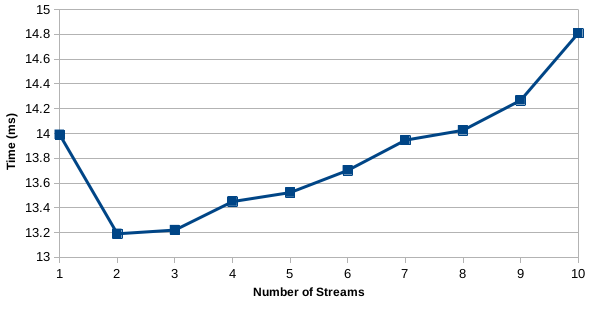
\includegraphics[width=\linewidth]{streamnumber.png}
  \caption {\textbf{The execution time of the program depending on the number of streams}}
  \label{fig:streamnumber}
\end{center}

\noindent A stream size of \code{2} seemed to yield the best overall execution time, and increasing the size further resulted in a worse performing program. This is likely due to the overhead involved in context switching outweighing the potential speedup increase. The execution time of the shaders remained relatively the same between all versions (averaging at around 2.84ms), which was expected as streaming mainly affects memory copying times. \\


\subsection{Pinned Memory}

\noindent While researching other solutions, we thought that looking into pinned memory could provide a possible decrease in execution time. Theoretically, it should have improved our execution times by preventing the need for paging\cite{pinnedmemory}. We modified our \hyperref[sec:V06]{V06} solution (\textit{V06 - Streams (mallocHost)} in the repository) to use \code{cudaMallocHost}, and this resulted in an average execution time of 68.80ms, with both shaders taking 30.378ms to run. We were surprised by this, as we were expecting better times, not significantly worse. It is possible we missed a caveat or did not implement it correctly, but we unfortunately did not have time to investigate this further. \\


\section{Conclusion}

\noindent After reviewing the results, we saw the significance that small changes to the program could bring. Simply porting a sequential program to CUDA already proved to be beneficial, and taking it steps further by being aware of how memory is stored and accessed was a very educational experience. We can see the importance of parallel computing, especially in real time applications such as real time rendering. We are relatively satisfied and confident with our results, having been able to bring the execution of the program with a moderately sized image from 206.89ms down to 13.19ms, despite shortcomings due to time constraints. \\ 


\section{Future Work}

\noindent Other potential investigations we could have performed to improve our execution time would have been to reorganize our data to prevent memory bank conflicts. While this could be easily done for the color correction algorithm, this proved too difficult for the blurring algorithm as it requires neighboring texels. If we had more time, we could have potentially looked into a way to organize memory to allow for an easier time calculating the offsets inside the shader itself. \\

\noindent Another possible approach would have been to unroll our loops, which could be tricky in practice due to the edges of the image requiring care to prevent accessing out of bounds memory. A possible solution would be to implement two solutions, one which only executes on the edges of the image and the rest which executes in the "safe zone", with the for loop unrolled. It would be interesting to measure whether the overhead of having to launch more shaders would have outweighed the performance improvements of performing jumps due to the loops.\\


\printbibliography

\end{document}